\documentclass{article}

\title{EECS E6892 Bayesian Models for Machine Learning\\ Homework 1}
\author{John Min; jcm2199}
\usepackage[margin=0.5in]{geometry}
\usepackage{amssymb, amsmath, parallel, mathtools, graphicx, array, pdfpages}\usepackage[T1]{fontenc}
\usepackage[scaled]{beramono}
\usepackage{listings}

\DeclareMathOperator{\Tr}{Tr} 


\begin{document}
\maketitle

\section{Expectation Maximiation (E.M.) of Probabilistic PCA}
$\{x_1, \ldots, x_N\} \in \mathcal{R}^d, x_n \sim N(W z_n, \sigma^2 I), W \in \mathcal{R}^{d \times k}$.  $W$ is unknown and $z_n \sim N(0, I)$.

\subsection{Compute posterior of z}
\begin{align*}
\displaystyle p(x_1, \ldots, x_N | W^{\text{old}}) & \propto p(x_1, \cdots, x_N | W^{\text{old}}, z_1, \cdots, z_N) p(z_1, \ldots, z_N) \\
& = \prod_{n=1}^N \Bigg[\exp \bigg\{\frac{(x_n - W^{\text{old}} z_n)^\top (x_n - W^{\text{old}} z_n) }{2 \sigma^2}\bigg\} \exp \bigg\{\frac{z_n^2}{2}\bigg\}\Bigg] \\
& \propto \exp \Bigg\{-\frac{1}{2} \sum_{n=1}^N \bigg[ z_n^\top z_n + \frac{1}{\sigma^2} z_n^\top W_{\text{old}}^\top W_{\text{old}} z_n - \frac{2}{\sigma^2} x_n^\top W_{\text{old}} z_n \bigg] \Bigg\}  \\
& = exp \Bigg\{-\frac{1}{2 \sigma^2} \sum_{n=1}^N \bigg[ z_n^\top \Big(\sigma^2 I + W_{\text{old}}^\top W_{\text{old}}) z_n - 2 x_n^\top W_{\text{old}} z_n \bigg] \Bigg\} \\
& \sim \mathbf{N(\mu, \Sigma)} \\
&\mathbf{\mu} = \bigg(\frac{\sigma^2 I + W_{\text{old}}^\top W_{\text{old}}}{\sigma^2 I} \bigg)^{-1} W_{\text{old}}^\top X \\
&\mathbf{\Sigma} = \frac{\sigma^2 I}{\sigma^2 I + W_{\text{old}}^\top W_{\text{old}}}
\end{align*}

\noindent
Note: \\
$- \frac{1}{2} (x - \mu)^\top \mathbf{\Sigma}^{-1} (x-\mu) = -\frac{1}{2} x^\top \mathbf{\Sigma}^{-1} x + x^\top \mathbf{\Sigma}^{-1} \mu +$ const. \\

\noindent
Above,
$\mu = x^\top W \\
z^\top \mathbf{\Sigma}^{-1} \mu = z^\top W^\top x \Rightarrow \mathbf{\Sigma}^{-1} \mu = W^\top x$

\subsection{Take expectation of complete data log-likelihood}
\begin{align*}
\displaystyle  &\mathrm{E}_{z_n} \Bigg[ \ln p \big(x_1, \ldots, x_N | W, z_1, \ldots, z_N \big)\Bigg] = \sum_{n=1}^N \Bigg[ \exp\big\{\frac{x_n^2}{2} \big\} - 2 \mathrm{E} \big[ x_n^\top W z_n \big] + \mathrm{E} \big[ z_n^\top W^\top W z_n\big] + \sigma^2 \mathrm{E} \big[ z_n^\top z_n \big] \Bigg] \\
& =\sum_{n=1}^N \Bigg[ \exp\bigg\{\frac{x_n^2}{2} \bigg\} -2 x_n^\top W \mu + \mathrm{E} \Big[(Wz_n)^\top (Wz_n)\Big] + \sigma^2 \big(\mu^2 + \Sigma \big) \Bigg] \\
& = \sum_{n=1}^N \Bigg[ \exp\bigg\{\frac{x_n^2}{2} \bigg\} - 2 x_n^\top W \mu + \big[\Tr(\mu^2 + \Sigma)\big]^\top \big[\Tr(WW^\top) \big] + \sigma^2 \big(\mu^2 + \Sigma \big)  \Bigg]
\end{align*}

\subsection{Maximize $Q(W, W^{\text{old}}) \text{ w.r.t. } W$}
Find the gradient with respect to W and set to 0: \\
$\displaystyle \sum_{n=1}^N \Big[ -2x_n^\top\mu + 2\Tr(\mu^2 + \Sigma)W = 0$.
(Note:  $\nabla_A \Tr(AB) = B^\top$). \\
$W^*$ aka $W^{\text{new}} = \Big[\Tr(\mu^2 + \Sigma) \Big]^{-1} \bar{X}^\top \mu$ where $\bar{X} = \frac{1}{N} \sum_{n=1}^N x_n$
\section{Implementation of Probabilistic Matrix Factorization}
\subsection{Maximum a posteriori (MAP)}
Update steps: \\
$u_i^{\text{MAP}} = \big(\lambda \sigma^2 I + V_i^\top V_i \big)^{-1} V_i^\top m_{u_i}$\\
$v_j^{\text{MAP}} = \big(\lambda \sigma^2 I + U_j U_j^\top \big)^{-1} U_j^\top m_{v_j}$\\

\noindent
Coordinate ascent is used for this MAP implementation where each update step for a particular $u_i$ optimizes the joint log-likelihood for $u_i$, and the update step for $v_j$ does the same for each $v_j$.  Each update step, whether it be for $u_i$ or for $v_j$ is an $\mathcal{L}_2$ regularized least squares solution, also known as ridge regression.
\subsection{Gibbs sampling}
Sample:
$u_i \sim N(\mu_i, \Sigma_i)$ where $\mu_i = \big(\lambda \sigma^2 I + V_i^\top V_i \big)^{-1} V_i^\top m_{u_i}$, $\Sigma_i = \big(\sigma^2 I + V_i^\top V_i \big)^{-1}$ \\
$v_j \sim(N(\mu_j, \Sigma_j)$ where $\mu_j = \big(\lambda \sigma^2 I + U_j U_j^\top \big)^{-1} U_j^\top m_{v_j}, \Sigma_j = \big(\sigma^2 I + U_j U_j^\top \big)^{-1}$\\

\noindent
A burn-in period of 250 iterations is used after which we collect samples every 25 iterations.  In each iteration, we sample each $u_i$ from the posterior distribution with parameters that are being updated for each $i$.  Then, we repeat for the $v_j$'s.

\subsection{Similar Movies by $v_j$ using d=10}
\subsubsection{Desperate Measures (1998)}
Doors, The (1991);
Mary Shelley's Frankenstein (1994);
Malice (1993);
Bye Bye, Love (1995);
Love Affair (1994).

\subsubsection{Oliver \& Company (1988)}
Indian in the Cupboard, The (1995);
Prefontaine (1997);
Abyss, The (1989);
Kid in King Arthur's Court, A (1995);
Air Up There, The (1994).

\subsubsection{Chinatown (1974)}
Manhattan (1979);
8 1/2 (1963);
Short Cuts (1993);
Annie Hall (1977);
Bonnie and Clyde (1967);


\subsection{Plots of results}

\begin{center}
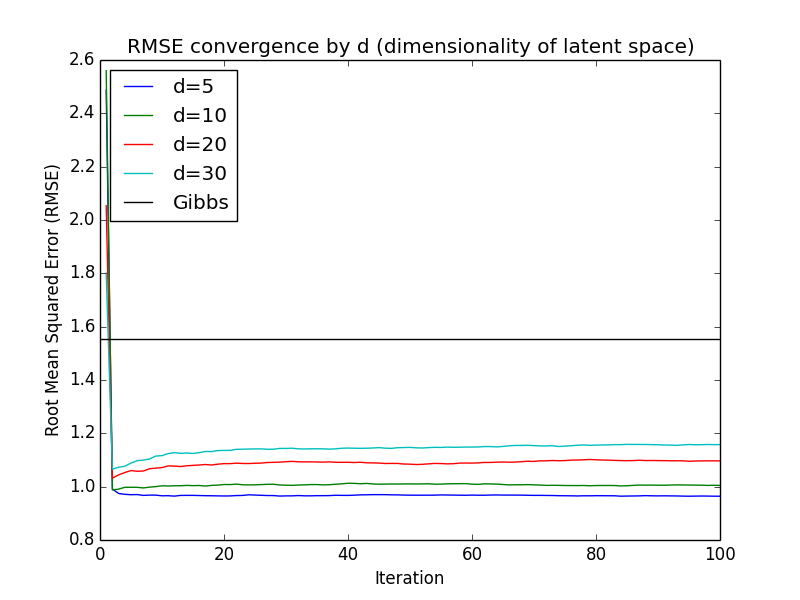
\includegraphics[scale=0.75]{RMSE.png}
\end{center}

\noindent
\begin{center}
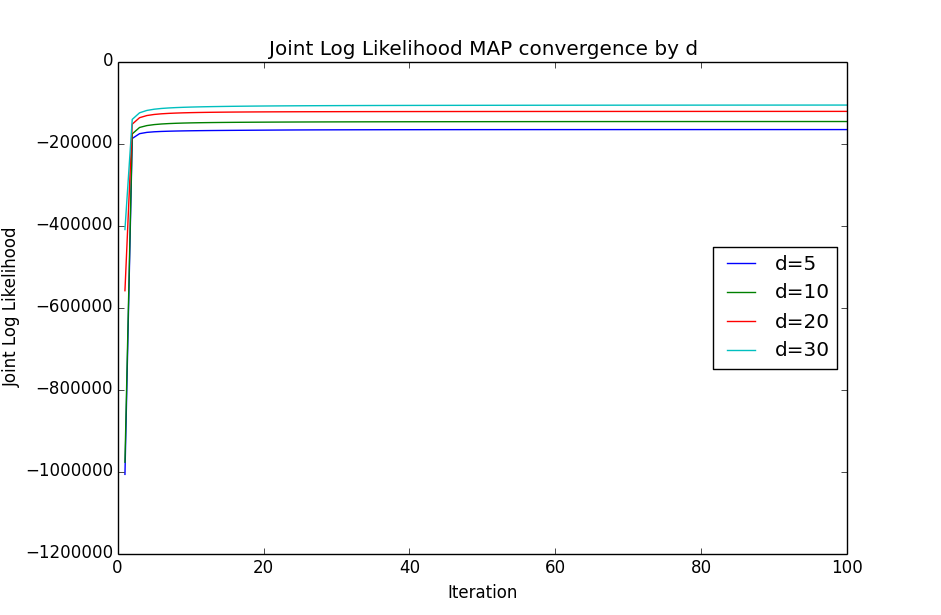
\includegraphics[scale=0.65]{LogJLL.png}\\
\end{center}

\noindent
\begin{center}
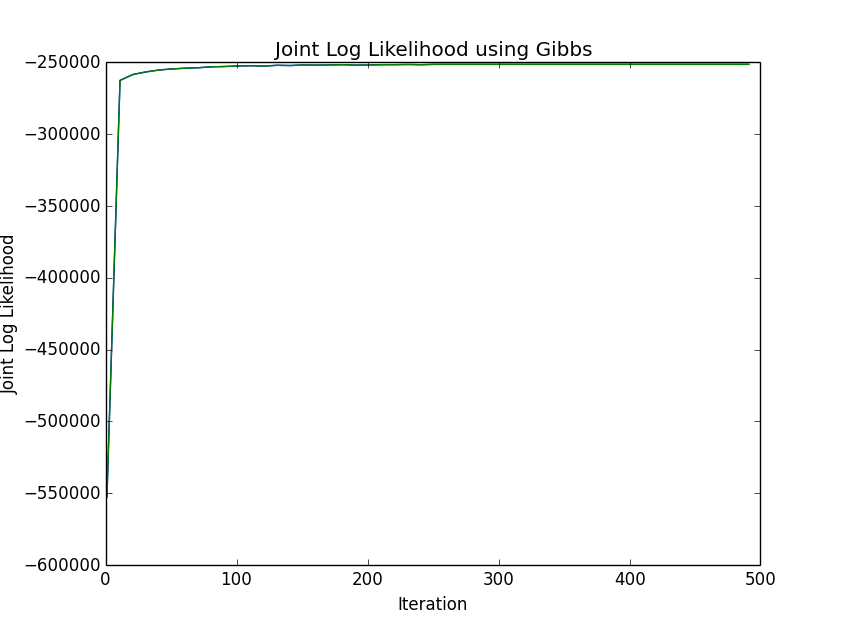
\includegraphics[scale=0.75]{JLL_Gibbs.png}\\
\end{center}

\newpage
\subsection{PMF - Python code}

\renewcommand*\familydefault{\ttdefault}
\lstset{
language=Python,
showstringspaces=true,
formfeed=\newpage,
tabsize=4,
commentstyle=\itshape,
basicstyle=\ttfamily,
morekeywords={models, lambda, forms}
}
 
\newcommand{\code}[2]{
\hrulefill
\subsection*{#1}
\lstinputlisting{#2}
\vspace{2em}
}
\lstinputlisting{./matrix_complete_MAP.py}


\end{document}